In der Erkennung von Hindernissen mithilfe von passiv optischen Systemen können verschiedenste Faktoren der Grund für eine fehlerhafte Erkennung sein. Sei es die Berechnung einer Disparity Map von Bereichen mit einer Vielzahl homogener oder reflektierender Flächen oder die Veränderung der Lichtverhältnisse in einem der beiden Kamerabilder. In diesem Kapitel werden einige der bestehenden, sowie einige potentiell mögliche Fehlerquellen erläutert sowie dazugehörige Lösungsansätze entwickelt.\\

% TODO Zusammenfassung Kapitel

% ---------------------- section -----------------------
\section{Bestehende Konflikte und Lösungsansätze}
\label{sec:existing_conflicts}

Die Validierung der erkannten Hindernisse ist ein kompliziertes Problem in der autonomen Hinderniserkennung. Durch etwaige äußere Einflüsse wie die Veränderung der Lichtverhältnisse kann die Berechnung der Tiefenkarte fehlerhaft sein. Dies kann im Fall eines autonomen Flugs dazu führen, dass das UAV ein Hindernis innerhalb eines Korridors erkennt und aufgrund dessen versucht diesem imaginären Hindernis auszuweichen. Gerade in engen Umgebungen ohne viel verfügbaren Platz kann dies zum totalen Systemausfall führen. Daher sollte ausgewertet werden ob es sich bei erkannten Hindernissen auch um solche handelt. Ein Ansatz zur Vermeidung solcher Falscherkennungen wäre, die Objekte insofern zu verfolgen, dass für jeden Frame (in Abhängigkeit der zugrundeliegenden Framerate) überprüft wird ob bereits im vorherigen Frame ein Objekt gefunden wurde. Erst nachdem dies sichergestellt wurde wird daraufhin eine Warnung ausgegeben. Zeitgleich wäre es möglich, dass Informationen wie die Eigenbewegung sowie die Information ob sich das erkannte Objekt selber im Raum bewegt verloren gehen.\\

\noindent
Eine andere Problematik stellt die Erkennung von homogenen, spiegelnden sowie durchsichtigen Flächen dar. Aufgrund fehlender Texturen sowie vorhandener Pixeldifferenzen kann die Korrespondenz zweier Pixel unter Umständen nicht bestimmt werden. Diese homogenen Bereiche haben demnach fehlerhafte Informationen zur Folge, so kann  einerseits einem Pixel an einer weißen Wand kein zugehöriger Pixel zugeordnet werden, andererseits ist es auch möglich das falsche Bildpunkte miteinander gematcht werden, welche wiederum eine hohe Disparität zur Folge haben. In diesem Fall wird ein Hindernis erkannt obwohl sich keines an dieser Position befunden hat. Abbildung \ref{fig:disparity-error-homogeneous} zeigt deutlich in welchen Bereichen der \emph{SGBM} aufgrund fehlender Textur keine Korrespondenzen finden konnte.\\

\begin{figure}[h]
	\centering
	\begin{tabular}{m{6.5cm} m{6.5cm}}
	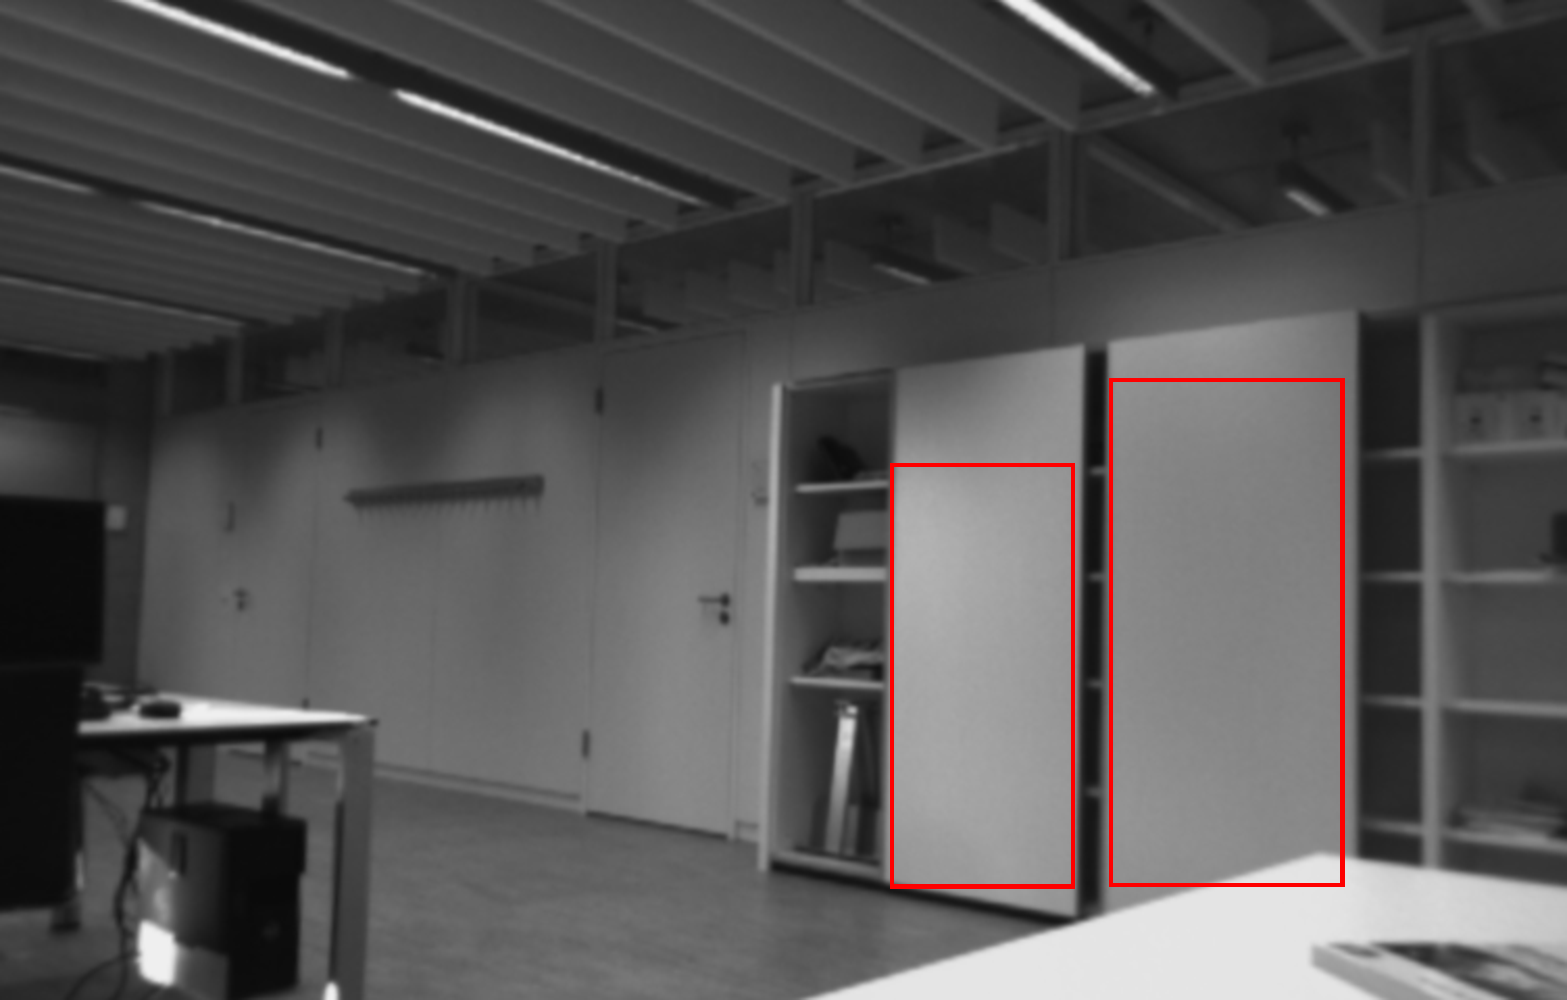
\includegraphics[width=6.5cm]{img/disparity_error_left.pdf}
	\begin{center} \small (a) linkes Kamerabild\end{center}
	&
	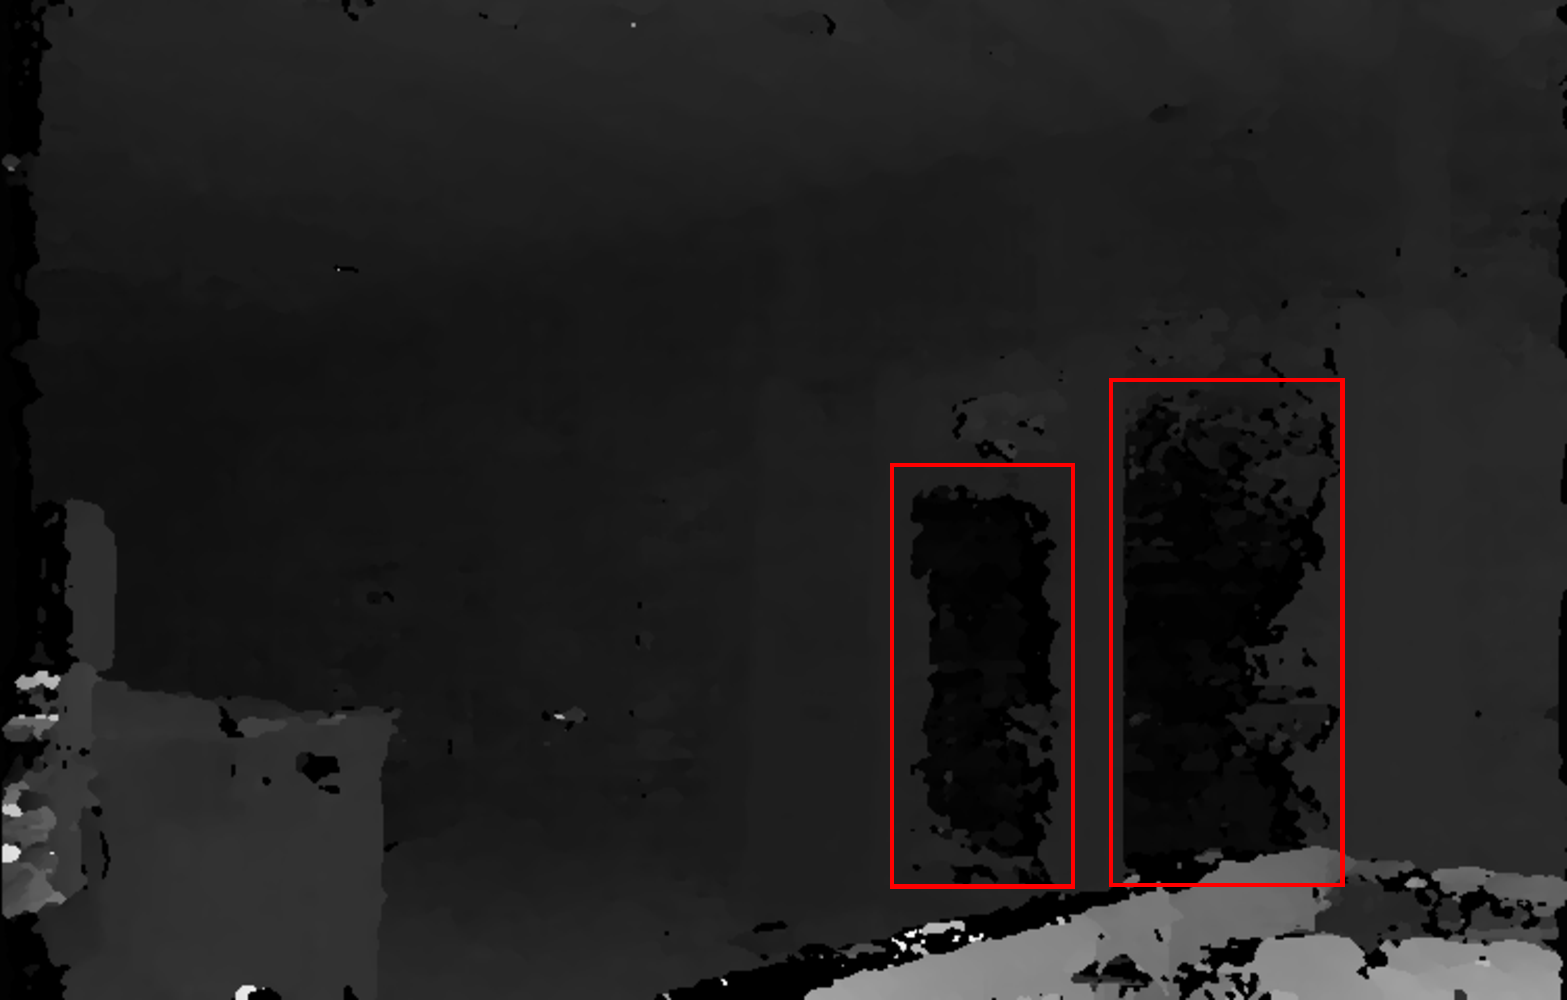
\includegraphics[width=6.5cm]{img/disparity_error.pdf}
	\begin{center} \small (b) Disparity Map \end{center}
	\end{tabular}
\caption{Konflikt in der Berechnung der Disparität bei nicht texturierten Flächen. Die in rot markierten Flächen sind das Resultat fehlender Texturierung.}
\label{fig:disparity-error-homogeneous}
\end{figure}

\noindent
Auch spiegelnde Flächen sind eine optische Problemstellung. Aufgrund der Projektion eines anderen Bereiches kommt es zu falschen Informationen innerhalb der Disparity Map. Hindernisse können zwar erkannt werden sofern sich die spiegelnde Fläche in einer günstigen Position befindet. Dies ist der Fall, wenn beide Kameras exakt den selben Bereich erfassen. Jedoch wird auch in diesem Fall eine weiter entfernte Distanz wahrgenommen anstelle des eigentlichen Objektes. Ist dies nicht der Fall so kann auch im Fall spiegelnder Flächen keine Disparität und folglich keine Tiefe wahrgenommen werden.\\
    % TODO Grafik spiegelnde Flächen
\noindent
Eine weitere Fehlerquelle sind durchsichtige Bereiche. Diese vereinen zum einen Fehlerquellen welche auch bei spiegelnden Arealen auftreten, zum anderen werden Objekte die sich hinter einer Glasscheibe befinden zwar erkannt (sofern keine Reflexion vorliegt) jedoch das Glas als eigentliches Hindernis nicht. Weiterhin besteht die Möglichkeit, dass Reflexionen aus Perspektive der beiden Kameras betrachtet einen anderen Tiefeneindruck vermitteln. Objekte werden so entweder weiter entfernt oder auch in kürzerer Distanz erkannt als sie sich wirklich befinden.\\

\noindent
Aufgrund des Aspektes, dass die Erkennung des Systems auf den Gebrauch in Innenbereichen konzipiert ist, gibt es verschiedenste Probleme bei der Anwendung in Außenbereichen. Zum einen ist die Verschlusszeit der Kameras fixiert. Die Verwendung einer automatischen Belichtungszeit ist nur für jede Kamera einzeln möglich. Um mit verschiedenen Lichtverhältnissen umgehen zu können, ohne dabei die Möglichkeit der Korrespondenzanalyse zu verlieren, muss die Verschlusszeit daher bei beiden Kameras immer gleich sein. Weiterhin ist die Erkennung des Bodens ein zu betrachtender Aspekt. Dieser ist bei aktueller Berechnung ein Teil der zu betrachtenden Hindernisse, was einerseits seine Berechtigung hat, andererseits auch bei niedrigen Flughöhen zu einer fehlerhaften Erkennung als Hindernis führt. 
	% TODO Hindernisgröße einbauen


% ---------------------- section -----------------------
\section{Diskussion}
\label{sec:conflict_discussion}
Ein Ansatz erkannte Hindernisse zu validieren ist, sich auf die letzte bekannte Position des Objektes zu berufen und im nächsten Einzelbild zu überprüfen ob es sich noch immer an selber Stelle befindet. Dabei würde für jedes Subimage/ jeden Samplepoint ausgewertet werden ob sich das Hindernis noch innerhalb dessen befindet. Jedoch schränkt dies die Erkennung bewegter Objekte stark ein. Ist die Geschwindigkeit eines Hindernisses so hoch, das in mindestens zwei aufeinanderfolgenden Frames kein Objekt im selben Subimage/Samplepoint erkannt werden kann so würde das System kein Hindernis erkennen können. Diese Methode ist daher prinzipiell mögliche jedoch stark von der Framerate sowie der eigenen bzw. Bewegung des Objektes abhängig. Grundlegend ist das System aufgrund der Beschaffenheit der Subimages für die Mean Disparity Detection geeignet, da die Größe der Subimages eine solche Validierung zulassen würde. Im Falle der Samplepoint Detection müssten auch die unmittelbar benachbarten Messpunkte mit einbezogen werden sodass die Bewegung auch verfolgt werden kann. Eine Kombination von Feature Tracking wäre dabei hilfreich, jedoch sehr rechenaufwändig.
    % paper suchen

Um auch die Erkennung homogener Flächen gewährleisten zu können besteht die Möglichkeit die Szene mithilfe externer Lichtquellen auszuleuchten um eine Texturierung zu erzwingen. Mit Hilfe eines Lasers würde dabei ein zufälliges Punktmuster auf die Szene projiziert werden, durch welches es dem Matching Algorithmus möglich ist korrespondierende Punkte innerhalb eines nicht texturierten Bereiches zu finden. Die Zufälligkeit der Punktwolke ist dabei ein wichtiges Kriterium, da die Gleichmässigkeit eines Rasters zu falschen Korrespondenzen führen könnte. Die Anwendung dieses Verfahrens ist jedoch hauptsächlich in Innenbereichen möglich, da die zu erkennenden Entfernungen unter Betrachtung der Einzelbild-Auflösung eine Detektion dieser zulassen würden. In Aussenbereichen ist es prinzipiell schwer Hindernisse aufgrund anderer Lichtverhältnisse ausfindig zu machen. Für diesen Anwendungsfall würde sich eine Berechnung homogener Flächen auf Matching Ebene anbieten. 

Der von Geiger et al. \cite{geiger2011efficient} entwickelte Matching Algorithmus...

% spiegelnd und reflektierend
Der von Tsin et al. \cite{tsin2003stereo} entwickelte Stereo Matching Algorithmus erkennt 

% glas ... keine ahnung meh
% Hindernisgroesse: ...meh
% aussenbereiche: autofokus meh,
\noindent
Ein weiterer bereits in Abschnitt \ref{sec:existing_conflicts} angeschnittener Punkt ist die Erkennung des Bodens als Hindernis. Dabei stellt sich die Frage ob eine Erkennung als Hindernis gewünscht ist oder nicht. Im Falle einer geringen Flughöhe wird der Boden ebenfalls als Hindernis erkannt. Dies kann einerseits eine Absicherung sein das die durch interne Sensoren ermittelte Flughöhe korrekt ist, andrerseits kann es dazu führen, dass der Algorithmus zur Vermeidung von Hindernissen versucht dieses zu  umgehen. Dies könnte unter Umständen dazu führen, dass das UAV eine Flughöhe annimmt welche über der, durch die Umgebung gegebenen, maximalen Flughöhe liegt. Eine mögliche Lösung wäre die Erkennung des Bodens in Abhängigkeit der aktuellen Höhe zu gestalten. Sollte sich das UAV unter der zur Erkennung des Bodens nötigen Flughöhe befinden so wird diese deaktiviert und der Boden wird nicht weiter betrachtet. Sofern die Flughöhe die Erkennung des Bodens ausschließt wird dieser entfernt.
% boden - Hindernis oder nicht?
